\documentclass[10pt]{beamer}

\usepackage{pgf, tikz, verbatim, amsmath, pdfpages}
\usetikzlibrary{arrows,automata}
\usepackage[latin1]{inputenc}
\title{ARM Cortex-M4 Architecture and Instruction Set}
\author{M J Brockway}

\begin{document}
\maketitle

\begin{frame}
\frametitle{Block diagram}
\begin{figure}[!htb]
\begin{center}
\includegraphics[width=0.8\textwidth]{CortexM4Core.png}
\end{center}
\end{figure}
This diagram is from the \href{http://hesabu.net/kf5011/docs/DUI0553A_cortex_m4_dgug.pdf}{\textcolor{blue}{Cortex M4 Generic User Guide}}, published by ARM. \emph{Further reading}: Chapter 1
\end{frame}

\begin{frame}
\frametitle{Programmer's model}
Ref: \emph{Generic User Guide} section 2.1. Click the link above, or find it on the module home page.\\~\\

Processor modes 
\begin{itemize}
\item [main] stack - running application software. Limited access to some instructions, system timer. System is in this mode immediately after reset.
\item[handler] mode - handling as exception. Returns to thread mode after all exceptions handled.
\end{itemize}
~\\~\\
Stacks
\begin{itemize}
\item \emph{full descending}: Stack pointer is \emph{decremented} when an item is pushed on; the stack grows `downwards'
\item Two stacks: \emph{main} and \emph{process}; a special register controls which.
\end{itemize}
\end{frame}

\begin{frame}
\begin{center}
\includepdf[pages=-,pagecommand={\thispagestyle{plain}}]{regSet.png}
\end{center}
\end{frame}

\begin{frame}
\frametitle{Programmer's model}
Registers ...
\begin{itemize}
\item[R0-R12]  32-bit general-purpose registers for data operations. Avoid using higher regsiters for applicaton programming!
\item[R13] the stack pointer: \emph{main} or \emph{process} stack depending on setting in CONTROL register.
\item[R14] is the \emph{link register}(LR): stores the return information for subroutines, function calls, and exceptions.
\item[R15] is the \emph{program counter}: stores the address of the next instruction to be fetched.
\item[PSR] The \emph{program status register} contains information about status of last operationn. Bits 27-31 are the \emph{condition codes}; the ones we shall be most concerned with are
  \begin{itemize}
  \item[N]: the last operation produced an arithmetically \emph{negative} result
  \item[Z]: the last operation produced a \emph{zero} result
  \item[C]: the last operation produced a \emph{carry} (or \emph{borrow})
  \item[V]: the last operation produced an arithmetic \emph{overflow}
  \end{itemize}
\end{itemize}
\end{frame}

\begin{frame}
\frametitle{Programmer's model}
Registers (ctd)
\begin{itemize}
\item \texttt{\color{blue}CONTROL} manages privilege level of the current instruction, and which of the two stacks to use.
\end{itemize}

Exceptions and interrupts
\begin{itemize}
\item[NVIC] The processor and the \emph{nested vectored interrupt controller} manage prioritized handling.
\end{itemize}
~\\
Data types
\begin{itemize}
\item 32-bit \emph{words}, 16-bit \emph{halfwords}, 8-bit \emph{bytes}.
\item Can be big- or little-endian;
\item instruction memory and private peripheral but (PPB) accesses are always little-endian. 
\end{itemize}

\end{frame}

\begin{frame}
\frametitle{Memory model}
\begin{columns}
  \begin{column}{0.5\textwidth}
  \begin{itemize}
  \item Ref: Generic User Guide sec 2.2;
  \item With 32-bit addressing, the memory space is 4 Gb.
  \end{itemize}
  \end{column}
 
  \begin{column}{0.5\textwidth}
  \includegraphics[height=0.9\textheight]{memMap.png}
  \end{column}
\end{columns}
\end{frame}

\begin{frame}
\frametitle{Memory model}
\begin{itemize}
\item \texttt{\color{blue}code} 00000000-1FFFFFFF is where executible code goes. On-chip FLASH. Data can go here, but not recommended.
\item \texttt{\color{blue}SRAM} 20000000-3FFFFFFF is primarily for application data, but code can go here.
\item \texttt{\color{blue}peripherals} 40000000-5FFFFFFF - on-chip peripherals
\item \texttt{\color{blue}external RAM} 60000000-9FFFFFFF - eg DDR, FLASH, LCD
\item \texttt{\color{blue}external device} A0000000-DFFFFFFF - external peripherals
\item \texttt{\color{blue}private peripheral bus} E0000000-E00FFFFF
\item \texttt{\color{blue}vendor-specific} E0100000-FFFFFFFF
\end{itemize}
\end{frame}

\begin{frame}
\frametitle{Cortex-M4 Image of a Program}
From low to high memory, ...
\begin{enumerate}
\item Interrupt vector table - addresses of interrupt and exception handlers
\item C startup routine
\item Application code and data
\item C library code 
\end{enumerate}

On reset, the CPU
\begin{enumerate}
\item Reads initial `stack pointer' address
\item Reads interrupt vector for `reset'
\item The reset handler branches to start of application program
\item The program executes ... 
\end{enumerate}
\end{frame}

\begin{frame}
\frametitle{Introducing Cortex-M4 Machine Instructions}
Reading: GUG chapter 3
\begin{itemize}
\item The size of most instructions is 32 bits (4 bytes) or 16 bits (2 bytes), comprising a \emph{THUMB-2 operation code} and sometimes and additional \emph{operand}.
\item The program as loaded into RAM is thus and array of 32-bit words. The address of the $n^{th}$ instruction (counting from 0) is therefore the base address of the loaded program + $32n$.
\item Shall use \emph{ARM assembly language} as a human-readable version of these instructions.   
\item The following is a simple program: simpler than 'Hello world', as it does not do any I/O. It simply uses registers R0, R1 to compute $10+9+8+...+1$, leaving the result in register R1.
\end{itemize}
\end{frame}

\begin{frame} [fragile]
\frametitle{Cortex-M4 Machine Instructions - simple example}
\small {
\begin{verbatim}
     PRESERVE8 ; Indicate the code here preserve 
               ; 8 byte stack alignment
     THUMB     ; Indicate THUMB code is used
     AREA    |.text|, CODE, READONLY   ; Start of CODE area
     EXPORT __main
     ENTRY
__main     FUNCTION
     ; initialize registers
     MOV  r0, #10  	; Starting loop counter value
     MOV  r1, #0   	; starting result
     ; Calculating 10+9+8+...+1 ...
loop
     ADD  r1, r0   	; R1 = R1 + R0
     SUBS r0, #1   	; Decrement R0, update flag ('S'   suffix)
     BNE  loop    	; If result not zero jump to loop
     ; Result is now in R1
deadloop
     B   deadloop  	; Infinite loop
     ENDFUNC
     END            ; End of file
\end{verbatim}
}
\end{frame}

\begin{frame} [fragile]
\frametitle{Simple example: pseudocode}
\small {
\begin{verbatim}
main function:
    Put value 10 in register 0
    Put value 0 in register 1
    Repeat:
        Add contents of R0 to R1, leaving result in R1;
        Subtract 1 from contents of R0, updating
                  condition codes according to the result;
        Check condition codes:
                  if 'Z' not set, repeat, else drop out of loop
    Forever run on the spot (branch to self)
\end{verbatim}
}
\end{frame}

\begin{frame} [fragile]
\frametitle{Simple example with machine code and relative addresses}
\small {
\begin{verbatim}
    1 00000000                 PRESERVE8      
    2 00000000         ; 8 byte stack alignment
    3 00000000                 THUMB           
    4 00000000                 AREA            
    5 00000000                 EXPORT           __main
    6 00000000                 ENTRY
    7 00000000         __main  FUNCTION
    8 00000000         ; initialize registers
    9 00000000 F04F 000A       MOV              r0, #10
   10 00000004 F04F 0100       MOV              r1, #0 
   11 00000008         ; Calculating 10+9+8+...+1
   12 00000008         loop
   13 00000008 4401            ADD              r1, r0 
   14 0000000A 3801            SUBS             r0, #1 
   15 0000000C D1FC            BNE              loop 
   16 0000000E         ; Result is now in R1
   17 0000000E         deadloop
   18 0000000E E7FE            B                deadloop 
   19 00000010                 ENDFUNC
   20 00000010                 END         
\end{verbatim}
}
\end{frame}

\begin{frame}
\frametitle{MOV, MVN}
Syntax
\begin{itemize}
\item \texttt{MOV}\{\texttt{S}\}\{\textit{cond}\} Rd, operand2
\item \texttt{MOV}\{\textit{cond}\} Rd, \#\textit{imm16}
\item \texttt{MVN}\{\texttt{S}\}\{\textit{cond}\} Rd, operand2
\item The \texttt{MOV} instructons copy the value of the second operand to Rd; \texttt{MVN} copies the \emph{complement} of this value to Rd.
\end{itemize}

where:
\begin{itemize}
\item \texttt{S} is an optional suffix. If included, the condition code flags are updated on the
 result of the operation.
\item \textit{cond} is an optional condition code (see below).
\item Rd is the destination - always a register.
\item operand2 is a flexible second operand: one of
  \begin{itemize}
  \item a constant: \#\textit{const} where 32-bit \textit{const} is either a left-shifted byte or a constant of one of the forms \texttt{00XY00XY}, \texttt{XY00XY00}, \texttt{XYXYXYXY}.
  \item a register with optional shift.
  \end{itemize}
\item \textit{imm16} is any value in the range 0-65535.
\end{itemize}
\end{frame}

\begin{frame}
\frametitle{MOV, MVN - Examples}
\begin{itemize}
\item \texttt{\color{brown}MOV R3, \#0x1F0000} - R3 set to 0x1F0000
\item \texttt{\color{brown}MVN R3, \#0x1F0000} - R3 set to 0xFFE0FFFFF
\item \texttt{\color{brown}MOV R3, R0} - value in R0 copied to R3
\item \texttt{\color{brown}MOVS R3, R0} - value in R0 copied to R3 and condition flags set according to result: Eg Z is set if result is 0; N is set if result is negative
\item \texttt{\color{brown}MVNS R3, R0} - complement of value in R0 copied to R3 and condition flags set according to result
\item \texttt{\color{brown}MVNSEQ R3, R0} - \emph{if Z is set} complement of value in R0 copied to R3 and condition flags set according to result
\end{itemize}

Some condition codes
\begin{itemize}
\item[EQ] \emph{equal}: Z==1
\item[NE] \emph{not equal}: Z==0
\item[HS] \emph{higher or same, unsigned}: C==1
\item[HI] \emph{higher, unsigned}: C==1 and Z==0
\item[GE] \emph{greater than or equal, signed}: N==V
\item[GT] \emph{greater than, signed}: N==V and Z==0
\end{itemize}

Exercise: Find definitions of LO, LS, LE, LT.
\end{frame}

\begin{frame}
\frametitle{Arithmetic}
Syntax
\begin{itemize}
\item \textit{op}\{\texttt{S}\}\{\textit{cond}\} \{Rd,\} Rn, operand2
\end{itemize}

where:
\begin{itemize}
\item \textit{op} is one of
  \begin{itemize}
  \item[ADD] - add: Rd $\leftarrow$ Rn + operand2
  \item[ADC] - add with carry: Rd $\leftarrow$ Rn + operand2 + C
  \item[SUB] - subtract: Rd $\leftarrow$ Rn - operand2
  \item[SBC] - subtract: Rd $\leftarrow$ Rn - operand2 - !C
  \item[RSB] - reverse subtract: Rd $\leftarrow$ operand2 - Rn
  \end{itemize}
\item Optional \texttt{S} suffix and \textit{cond} condition are as we defined above.
\item Rd, Rn are registers: Rd is the destination. Its specification is optional: if absent, Rd=Rn.
\item operand2 is a flexible second operand, a byte-sized immediate value or a register with optional shift (see GUG ch 3).
\item \texttt{ADD, SUB} also allow operand2 to be any value in the range 0-4095 (12 bits).
\item N,Z,C,V flags updated (with S option) according to result.
\end{itemize}
\end{frame}

\begin{frame}
\frametitle{Arithmetic Examples}
\begin{itemize}
\item \texttt{\color{brown}ADD R0, R1, R1, LSL \#2}: R0 $\leftarrow$ R1 + (R1 $<<$ 2)
\item \texttt{\color{brown}ADDEQ R0, R1, \#1} - If Z flag is set, R0 $\leftarrow$ R1 + 1
\item \texttt{\color{brown}ADDS R0, \#1} - R0 $\leftarrow$ R0 + 1
\item \texttt{\color{brown}ADC R3, R4, R5} - R3 $\leftarrow$ R4 + R5 + C
\item \texttt{\color{brown}SUBS R0, R0, \#1} - R0 $\leftarrow$ R0 - 1; update condition flags
\item \texttt{\color{brown}SBCNES R0, R1, R2} - If Z is clear, R0 $\leftarrow$ R0 - R2 - !C; update condition flags
\item \texttt{\color{brown}RSBS R0, R1} - R0 $\leftarrow$ R1 - R0; update flags
\end{itemize}
\end{frame}

\begin{frame}
\frametitle{Logic}
Syntax
\begin{itemize}
\item \textit{op}\{\texttt{S}\}\{\textit{cond}\} \{Rd,\} Rn, operand2
\end{itemize}

where:
\begin{itemize}
\item \textit{op} is one of
  \begin{itemize}
  \item[AND] - bitwise AND: Rd $\leftarrow$ Rn \& operand2
  \item[ORR] - bitwise OR: Rd $\leftarrow$ Rn | operand2
  \item[EOR] - bitwise exclusive OR: Rd $\leftarrow$ Rn \^ operand2
  \item[BIC] - bitwise AND NOT: Rd $\leftarrow$ Rn \& !(operand2); clears bits in Rb marked by operand2
  \item[ORN] - bitwise OR NOT: Rd $\leftarrow$ Rn | !(operand2)
  \end{itemize}
\item Optional \texttt{S} suffix and \textit{cond} condition are as we defined above.
\item Rd, Rn are registers: Rd is the destination. Its specification is optional: if absent, Rd is Rn.
\item operand2 is a flexible second operand, a byte-sized immediate value or a register with optional shift (see GUG ch 3).
\item With S option, N,Z updated according to result (possibly also C during evaluation of operand2) 
\end{itemize}
\end{frame}

\begin{frame}
\frametitle{Logic Examples}
\begin{itemize}
\item \texttt{\color{brown}ORREQ R0, R1, \#0x1F} - If Z is set, R0 $\leftarrow$ R1 | 0x1F
\item \texttt{\color{brown}EORS R0, R1} - R0 $\leftarrow$ R0 \^ R1; set flags
\item \texttt{\color{brown}BIC R3, R4} - R3 $\leftarrow$ R3 \& !R4: bits set in R4 are cleared in R3
\end{itemize}
\end{frame}

\begin{frame}
\frametitle{Shifts}
Syntax
\begin{itemize}
\item \textit{op}\{\texttt{S}\}\{\textit{cond}\} Rd, Rn, Rs
\item \textit{op}\{\texttt{S}\}\{\textit{cond}\} Rd, Rn, \#n
\item \texttt{RRX}\{\texttt{S}\}\{\textit{cond}\} Rd, Rn
\end{itemize}

where:
\begin{itemize}
\item \textit{op} is one of
  \begin{itemize}
  \item[ASR] - arithmetic shift right
  \item[LSL] - logical shift left
  \item[LSR] - logical shist right
  \item[ROR] - rotate right
  \end{itemize}
\item Optional \texttt{S} suffix and \textit{cond} condition are as we defined above.
\item Rd is the destination register; Rn is register holding the value to be shifted
\item Register Rs holds value of shift length - only the lowest order byte applies
\item \#n is a shift length:
  \begin{itemize}
  \item[ASR, LSR] $1 \le n \le 32$; 
  \item[LSL, ROR] $0 \le n \le 31$;
  \end{itemize}
\item \texttt{RXX} sets Rd to bits in Rn rotated right 1 bit.
\item With S option, N,Z updated according to result; if shift length $> 0$, C updated to last bit shifted out.
\end{itemize}
\end{frame}

\begin{frame}
\frametitle{Comparisons}
These always update the condition flags, without needing an \texttt{S} suffix. There is no destination register: the only purpose is to update the flags.\\
Syntax:
\begin{itemize}
\item \texttt{CMP}\{\textit{cond}\} Rn, operand2
\item \texttt{CMN}\{\textit{cond}\} Rn, operand2
\item \texttt{TST}\{\textit{cond}\} Rn, operand2
\item \texttt{TEQ}\{\textit{cond}\} Rn, operand2
\end{itemize}

where:
\begin{itemize}
\item Rn register holds the first operand;
\item operand2 is a flexible second operand, as seen above.
\item \texttt{CMP} subtracts the operands and \texttt{CMN} adds the operands, setting the condition flags but discarding the result. Cf \texttt{SUBS, ADDS}.
\item \texttt{CMP R0, R1} sets Z and C if R0==R1, sets N if R1 $>$ R0, sets C if R0 $>$ R1
\item \texttt{TST} bitwise ANDs the operands and \texttt{TEQ} bitwise EORs the operands, setting the condition flags but discarding the result. Cf \texttt{ANDS, EORS}.
\end{itemize}
\end{frame}

\begin{frame}
\frametitle{Branching}
\begin{itemize}
\item To do anything other than run a fixed sequence of instructions, the CPU needs to be able decide on the result of some test what instruction to execute next.
\item In normal operaton, an instruction is \emph{fetched} from the address pointed at by the \emph{Program Counter} (PC = R15), and the PC immediately incremented by the size of that instruction: 2  or 4 bytes. Then the ``next'' instruction is the next in the RAM.
\item A branch instruction overrides this by \emph{setting} the PC to some other value - some other valid instruction address, we hope. 
\item A \emph{conditonal} branch: only happens if some condition is met.
\item The ``next'' instruction to be fetched is the one whose address was loaded into the PC by the branch instruction.
\end{itemize}
\end{frame}

\begin{frame}
\frametitle{Branching}
Syntax
\begin{itemize}
\item \texttt{B}\{\textit{cond}\} label
\item \texttt{BL}\{\textit{cond}\} label
\item \texttt{BX}\{\textit{cond}\} Rm
\item \texttt{BLX}\{\textit{cond}\} Rm
\end{itemize}

where:
\begin{itemize}
\item \textit{cond} is an optional condition code, \texttt{EQ, NE, LT, LE, GE, GT, ...} etc
\item Rm is a register containing the address to branch to.
\item A \emph{label} is declared in the assembly language code as an unindented symbol: eg \texttt{\color{blue}\_\_main}, \texttt{\color{blue}loop}, \texttt{\color{blue}deadloop} on slide 11
\end{itemize}
\end{frame}

\begin{frame}
\frametitle{Memory Access Instructions with immediate offset}
Syntax
\begin{enumerate}
\item {\color{brown}\textit{op}\{\textit{type}\}\{\textit{cond}\} Rt, [Rn]} - no offset or write-back
\item {\color{brown}\textit{op}\{\textit{type}\}\{\textit{cond}\} Rt, [Rn, \#\textit{offset}]} - immediate offset, no write-back
\item {\color{brown}\textit{op}\{\textit{type}\}\{\textit{cond}\} Rt, [Rn, \#\textit{offset}]!} - pre-indexed
\item {\color{brown}\textit{op}\{\textit{type}\}\{\textit{cond}\} Rt, [Rn], \#\textit{offset}} - post-indexed
\end{enumerate}

where:
\begin{itemize}
\item \textit{op} is one of
  \begin{itemize}
  \item[LDR] - load register Rt from [...]
  \item[STR] - store register Rt to [...]
  \end{itemize}
\item \textit{type} is one of
  \begin{itemize}
  \item[B] - unsigned byte (0-extended to 32 bits)
  \item[SB] - signed byte (on load, sign-extended to 32 bits)
  \item[H] - unsigned halfword (0-extended to 32 bits)
  \item[SB] - signed halfword (on load, sign-extended to 32 bits)
  \item omitted if whole word is to be loaded or stored
  \end{itemize}
\item Optional \textit{cond} condition is \texttt{EQ, NE, ...} as we defined above.
\item Rt is register to load to or store from.
\end{itemize}
\end{frame}

\begin{frame}
\frametitle{Examples}
\begin{itemize}
\item \texttt{\color{brown}LDR R8, [R10]} - load R8 from memory address R10
\item \texttt{\color{brown}STR R2, [R5, \#4]} - store R2 to memory address R5+4; value in R5 is unchanged
\item \texttt{\color{brown}LDR R2, [R5, \#4]!} - Add 4 onto contents of R5, then  load R2 from memory address R5
\item \texttt{\color{brown}STR R2, [R5], \#-4} - load R2 from memory address R5 then decrement contents of R5 by 4
\end{itemize}
\end{frame}

\begin{frame}
\frametitle{Data Definitions}
These instructions assume we have a register containing an address pointing at an item of data, or perhaps an array of data. One way this comes about is via the \emph{assembler directives} which define and reserve memory for data.\\
~\\
\{\textit{label}\} \texttt{DCD} \textit{expr}\{, \textit{expr}\} ...\\ 
\{\textit{label}\} \texttt{DCDU} \textit{expr}\{, \textit{expr}\} ... 
\begin{itemize}
\item defines a 32-bit word or a sequence of words with optional label giving address.
\item \textit{expr} is a numeric expression
\item The version \emph{without} \texttt{U} adds padding so that the data is aligned on a \emph{word boundary}, an address that is a multiple of 4. Usually the \emph{unaligned} version is the simpler one to use. 
\item Example
  \begin{itemize}
  \item \texttt{\color{brown}numArray DCDU 1000000, 999999, 999998, 999997}
  \end{itemize}
\item \texttt{\color{brown}LDR R0, =numArray} ;\emph{loads address of data into R0}
\item \texttt{\color{brown}LDR R1, [R0, \#4]} ;\emph{loads 999999 into R1} {\color{brown}Why \texttt{\#4}?} 
\end{itemize}
\end{frame}

\begin{frame}
\frametitle{The Cortex-M4 Stack}
\begin{center}
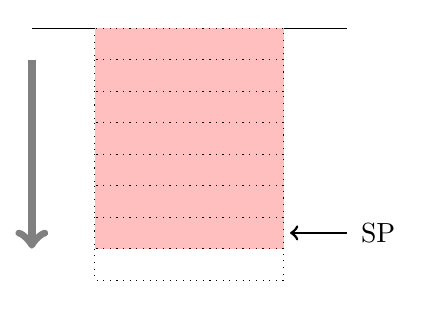
\begin{tikzpicture}[font=\normalsize, scale=0.04]
  \draw (0,80) -- (100,80);
  \fill[pink] (20,80) rectangle (80,10); 
  \draw[dotted] (20,80) rectangle (80,70); 
  \draw[dotted] (20,70) rectangle (80,60); 
  \draw[dotted] (20,60) rectangle (80,50); 
  \draw[dotted] (20,50) rectangle (80,40); 
  \draw[dotted] (20,40) rectangle (80,30); 
  \draw[dotted] (20,30) rectangle (80,20); 
  \draw[dotted] (20,20) rectangle (80,10); 
  \draw[dotted] (20,10) rectangle (80,0); 
  \draw[line width=3pt, gray, ->] (0,70) -- (0,10);
  \draw[line width=1pt, ->] (100,15) -- (82,15);
  \draw (110,15) node{SP};
\end{tikzpicture}
\end{center}
The subroutine stack is \emph{full, descending}
\begin{itemize}
\item It ``grows'' downwards from higher to lower memory addresses
\item The stack pointer \texttt{SP}, register R13, points at the last word on the stack.
\item \texttt{SP - 4} is address of next available space on the stack. 
\end{itemize} 
Alternatives
\begin{itemize}
\item ascending - ``grows'' upwards
\item empty - \texttt{SP} points at next available space rather than last occupied space. 
\end{itemize} 
\end{frame}

\begin{frame}
\frametitle{Full Descending Stack operations}
\begin{itemize}
\item[PUSH] Decrement SP, then store data to where SP points
\item[POP] Retrieve data from where SP points, then increment SP.
\end{itemize} 
(Questions: how would these be different for an ascending full stack? an ascending empty stack?)
\end{frame}

\begin{frame}
\frametitle{Full Descending Stack operations}
Cortex-M4 Syntax
\begin{itemize}
\item \texttt{PUSH}\{\textit{cond}\} \textit{regs-list}
\item \texttt{POP}\{\textit{cond}\} \textit{regs-list}
\end{itemize}

where:
\begin{itemize}
\item \textit{cond} is an optional condition code, as before: the operation occurs only if the condition is true
\item \textit{regs-list} is a comma-separated list in braces \{\} of regsters or ranges or registers (eg R0-R3, etc)
\item PUSH stores the register contents with higher-numbered registers at higher addresses, starting at \texttt{SP-4}. At the end, \texttt{SP} points at the lowest stored value.
\item POP loads the registers from the stack, assuming higher-numbered registers are at higher addresses, and post-increments \texttt{SP} by 4 times the number of registers popped.
\end{itemize}
\end{frame}

\begin{frame}
\frametitle{Full Descending Stack operations}
\begin{itemize}
\item Do not include the SP in the register list;
\item Special restrictions apply to including the PC in the register list.
\item You normally \emph{do} need to push th LR if you want to be able to nest subroutine calls.
\item These instructions do not change the condition code flags.
\end{itemize}

Examples
\begin{itemize}
\item \texttt{PUSH \{R0,R4-R7\}}
\item \texttt{PUSH \{R0-R2,LR\}}
\item \texttt{POP \{R5-R8\}}
\end{itemize}

Question: describe the effect of following the last two examples one after the other.
\end{frame}

\begin{frame} [fragile]
\frametitle{Subroutines - basic idea}
The black code contains a call to the function defined by the brown code:
\begin{verbatim}
    ....
    BL myFunc
    ....
\end{verbatim}
{\color{brown}
\begin{verbatim}
 myFunc FUNCTION
    ....
    ....; do some complicated stuff
    BX LR
    ENDFUNC
\end{verbatim}
}
\begin{itemize}
\item The {\color{brown}brown} code defines a function labelled \texttt{myFunc}
\item A branch to \texttt{myFunc} starts executing it.
\item The last thing \texttt{myFunc} does is \texttt{BX LR}: branch to the address stored in the link register...
\item ... so the calling code should brach with \texttt{BL myFunc} - branch to myFunc storing the return address in the link register. This is the PC value of the instruction \emph{after} \texttt{BL myFunc}.
\end{itemize}
\end{frame}

\begin{frame} [fragile]
\frametitle{Subroutines - example}
A simple function to compute largest (unsigned) integer $\le \sqrt x$: 
\color{brown}
\begin{verbatim}
typedef unsigned int uint32_t;

uint32_t usqt(uint32_t x) {
  uint32_t n = 0x8000,
           m = 0;
  while (n != 0) {
    m += n;
    if (m*m > x) {
      m -= n;
    }
    n >>= 1;
  }
  return m;
}
\end{verbatim}
\end{frame}

\begin{frame} [fragile]
\frametitle{Subroutines - example}
Here is an assembly language version: 
\begin{verbatim}
    1:     PRESERVE8 ; Indicate the code here preserve 
    2:               ; 8 byte stack alignment
    3:     THUMB     ; Indicate THUMB code is used
    4:     AREA    |.text|, CODE, READONLY  
    5:     EXPORT __main
    6:     ENTRY
    7: __main     FUNCTION
    8:     ; initialize registers
    9:     MOV  r0, #1000  	; Starting loop counter value
   10: 	  BL usqt
   11: deadloop
   12:     B   deadloop  	; Infinite loop
   13:     ENDFUNC
   14:
\end{verbatim}
\end{frame}

\begin{frame} [fragile]
\frametitle{Subroutines - example}
\color{brown}
\begin{verbatim}
   15: usqt       FUNCTION
   16:     ; compute highest 32-bit uint < value in r0
   17:     ; return  value in r0
   18:     PUSH {r1-r3}
   19:     MOV r1, #0x8000 ; n = 0x8000
   20:     MOV r2, #0      ; m = 0
   21: usqLoop
   22:     ADD r2, r2, r1  ; m += n
   23:     MUL r3, r2, r2  ; r3 = m*m
   24:     CMP  r3, r0
   25:     BLS  jump       ; if unsigned lower or same as x
   26:     SUB  r2, r2, r1 ; skip this step
   27: jump
   28:     LSRS r1, r1, #1
   29:     BNE usqLoop
   30:     MOV r0, r2      ; copy result into r2
   31:     POP {r1-r3}
   32:     BX LR
   33:     ENDFUNC	 
   34:     END             ; End of file
\end{verbatim}
\end{frame}

\begin{frame} [fragile]
\frametitle{Subroutines - example}
\begin{itemize}
\item Line 10 in the main function calls the subroutine function \texttt{\color{brown}usqt} with \texttt{BL usqt}
\item The function is actually defined on lines 15-33. You will need to satisfy yourself these are equivalent to the C code above.
\item Line 32 ends the function call with a branch to the address saved in LR by the line 10.
\item The function gets the parameter $x$ in register r0, uses registers r1, r2, r3 as ``local variables'' and returns the result in r0.
\item IT IS GOOD PRACTICE therefore to PUSH these registers onto the stack at the beginning (line 18) and restore them with a POP at the end of the call, line 31.
\item It is also common prctice to push LR onto the stack (and pop it off at the end) as well: ESSENTIAL if this function itself calls another function.
\item In fact, {\color{brown}push and pop all registers the function alters in any way}.
\item In this case, register r0 is excluded because it is used to pass the return value back to the calling code.  
\end{itemize}
\end{frame}

\begin{frame} [fragile]
\frametitle{Calling a subroutines from C - \texttt{main.c}}
\color{brown}
\begin{verbatim}
    1: int fact(int x);
    2: int x, y;
    3: 
    4: int main() {
    5: 	x = 4;
    6: 	y = fact(x);
    7: 	return 0;
    8: }
\end{verbatim}
\end{frame}


\begin{frame} [fragile]
\frametitle{Calling a subroutines from C - \texttt{factorial.c}}
{\small \color{brown}
\begin{verbatim}
    1:     PRESERVE8 ; Indicate the code here preserve 
    2:               ; 8 byte stack alignment
    3:     THUMB     ; Indicate THUMB code is used
    4:     AREA    |.text|, CODE, READONLY   ; Start of CODE area
    5:     EXPORT fact
    6:     ENTRY
    7: fact     FUNCTION
    8:     ; expects arg in R0; returns val in R0
    9:     PUSH {R1,R2, LR} ; save working registers and LR
   10:     MOVS  R1, R0  	 ; if nonzero, recursive call ... 
   11:     BNE recvCall     ; else ...
   12:     MOV R0, #1
   13:     B return
   14: recvCall
   15:     SUB R0, #1
   16:     BL fact
   17:     MUL R0, R0, R1
   18: return
   19:     POP {R1,R2, LR} ; restore saved registers
   20:     BX LR
   21:     ENDFUNC
   22:     END            ; End of file
\end{verbatim}
}
\end{frame}



\end{document}
